\documentclass{article}
\usepackage{amsmath}
\usepackage[margin=0.75in]{geometry}
\usepackage{graphicx}
\def\Omb{\Omega_\mathrm{b}}
\def\rhob{\rho_\mathrm{b}}
\def\rhocrit{\rho_\mathrm{crit}}
\def\nIGM{n_\mathrm{IGM}}
\def\rhoIGM{\rho_\mathrm{IGM}}
\def\mh{m_\mathrm{H}}
\def\kmsMpc{\mathrm{km/s/Mpc}}

\def\beq{\begin{eqnarray}}
\def\eeq{\end{eqnarray}}

\title{Baryon Imbalance}
\author{Andr\'{e}s N. Salcedo}
  
\begin{document}

\maketitle

The Big Bang should have created equal amounts of matter and antimatter and yet barely any antimatter is observed. Neither general relativity or the standard model offer explanations for this imbalance. This problem is referred to as the baryon asymmetry problem. One possible explanation is that matter and antimatter dominate different large scale regions of the universe. At astronomical distances matter and antimatter are indistinguishable but at the boundaries between these regions annihilation would occur offering an observational test of this theory. 

\begin{enumerate}

\item Estimate the number density of the IGM.

  We can approximate the density of the IGM by calculating the cosmological mean baryon density. We have by the Friedmann equation:

  \beq
  \rhoIGM \sim \rhob = \Omb \rhocrit = \Omb \frac{3 H^2}{8 \pi G}
  \eeq
  
  Approximating the IGM as all neutral hydrogen we have the number density:

  \beq
  \nIGM = \frac{\Omb}{\mh} \frac{3 H^2}{8 \pi G}
  \eeq
  
  Evaluating at order of magnitude, $\Omb = 0.04$, $H = 70 \; \kmsMpc$:

  \beq
  \nIGM \sim 2 \times 10^{-7} \; \mathrm{cm^{-3}}
  \eeq

\item Estimate the particle collision rate in the IGM, as well as the matter-antimatter collision rate assuming equal amounts of each.

  The mean free path is given by:

  \beq
  \mathit{l_\mathrm{IGM}} = \frac{1}{\nIGM \sigma} = \frac{1}{\nIGM \pi a^2} \sim 6 \times 10^{22} \; \mathrm{cm} \sim 20 \; \mathrm{kpc}
  \eeq

  Where we approximate neutral hydrogen as a sphere of the Bohr radius, $a$. We need the mean particle velocity in the IGM to calculate the collision rate. Assuming the IGM is in equilibrium with the CMB (applying the equipartition theorem for a monoatomic gas) we have:

  \beq
  v = \sqrt{\frac{3 k_\mathrm{b} T_\mathrm{CMB}}{\mh}} \sim 260 \; \mathrm{m/s}
  \eeq

  The particle collision rate is then:

  \beq
  r = \frac{v}{l_\mathrm{IGM}} \sim 4 \times 10^{-19} \; \mathrm{s^{-1}}
  \eeq

  We need to include a multiplicative factor of $2f(1 - f)$, where $f$ is the antimatter fraction, to get the matter-antimatter collision rate:

  \beq
  r \sim 2 \times 10^{-19} \; \mathrm{s^{-1}}
  \eeq

  A more useful quantity is the volumetric collision rate:

  \beq  
  \Gamma = \nIGM \times r \sim 4 \times 10^{-26} \; \mathrm{cm^{-3}} \; \mathrm{s^{-1}}
  \eeq
  
\item Assume that we are at the center of a spherical region of space dominated by matter. Write an expression for the gamma-ray surface brightness due to matter-antimatter annihilations (assuming equal matter and antimatter).

  The total number of photons produced in a infinitesimal volume per time is given by:

  \beq
  \frac{dN}{dt} = \Gamma \times 4 \pi r^2 dr
  \eeq

  So the intensity:

  \beq
  dI_{\nu} = \frac{dN}{dA \; dt \; d\Omega \; d\nu} = \frac{4 \pi \Gamma r^2 dr}{4 \pi r^2 \; dt \; 4 \pi \; d\nu} \sim \frac{\Gamma}{4 \pi} dr
  \eeq

  The final equality is made because our source is (basically monochromatic). Integrating for $I$:

  \beq
  I = \int_{r}^{r + \delta r} \frac{\Gamma}{4 \pi} dr' = \frac{\Gamma}{4 \pi} \delta r
  \eeq

  In this case the mean free path for collisions seems like a reasonable estimate for $\delta r$, and additionally since the sources are not isotropic but instead output two photons in opposite directions I $\emph{believe}$ we need an extra factor of $2 / 4 \pi$:

  \beq
  I = \frac{\Gamma}{ 8 \pi^2} l_{IGM} \sim 2.4 \times 10^{-5} \; \mathrm{cm^{-2}} \; \mathrm{s^{-1}} \; \mathrm{sr^{-1}} 
  \eeq

\item If we observed a radiation background of energy $3 \times 10^5 \; \mathrm{keV}$ of brightness, $I = 10^{-4} \; \mathrm{cm^{-2}} \; \mathrm{s^{-1}} \; \mathrm{sr^{-1}}$  that we could be pretty sure is from annihilation at a matter-antimatter boundary, what would this imply about the value of $\Omega_\mathrm{b}$ and the scale of our matter dominated region (again assume equal matter and antimatter)?

  The energy of the photons:

  \beq
  \epsilon = \frac{1}{2} m_h c^2 (1 + z)^{-1}
  \eeq

  \beq
  z = \frac{m_h c^2}{2 \epsilon} - 1 \sim 0.5 
  \eeq

  Applying equations 2, 4, 8, and 13 we have:

  \beq
  I = \frac{n_{IGM} v}{8 \pi^2} = 2.4 \times 10^{-5} \left( \frac{\Omega_b}{0.04} \right) \; \mathrm{cm^{-2}} \; \mathrm{s^{-1}} \; \mathrm{sr^{-1}}
  \eeq

  So if we observed $I = 10^{-4} \; \mathrm{cm^{-2}} \; \mathrm{s^{-1}} \; \mathrm{sr^{-1}}$ that would imply:

  \beq
  \Omega_b \sim 0.16
  \eeq

\item Based on the data given write an expression relating $\Omega_\mathrm{b}$, and the redshift the hypothesized boundary. If we take $\Omega_\mathrm{b} = 0.04$ what limiting distance to the hypothesized boundary does that require.

  Based on the attached plot the gamma-ray background spectrum appears to be consistent with a power-law, at least to order of magnitude. I estimate the power-law index to be about, $\gamma = -\frac{11}{5} \sim 2$, and taking the convenient value of $I(\epsilon = 1 \; \mathrm{keV}) = 10$ we can solve for the normalization factor:

  \beq
  I(\epsilon) = (10 \; \mathrm{cm^{-2}} \; \mathrm{s^{-1}} \; \mathrm{sr^{-1}}) \left( \frac{\epsilon}{\mathrm{keV}} \right)^{-2}
  \eeq

  With this relation we can at least put an upper bound on the gamma ray surface brightness due to matter-antimatter annihilations from our hypothesized large scale region boundary:

  \beq
  2.4 \times 10^{-5} \left( \frac{\Omega_b}{0.04} \right) \; \mathrm{cm^{-2}} \; \mathrm{s^{-1}} \; \mathrm{sr^{-1}} \leq (10 \; \mathrm{cm^{-2}} \; \mathrm{s^{-1}} \; \mathrm{sr^{-1}}) \left( \frac{\epsilon}{\mathrm{keV}} \right)^{-2}
  \eeq

  Taking $\frac{1}{2} m_h c^2 \sim 5 \times 10^5 \; \mathrm{keV}$ we have:

  \beq
  10^{-5} \geq \frac{1}{(1 + z)^2} \left( \frac{\Omega_b}{0.04} \right)
  \eeq

  Taking $\Omega_b = 0.04$ we get a very harsh constraint:

  \beq
  z \geq 10^{5/2} \sim 300
  \eeq

\end{enumerate}

\begin{figure}
\begin{center}
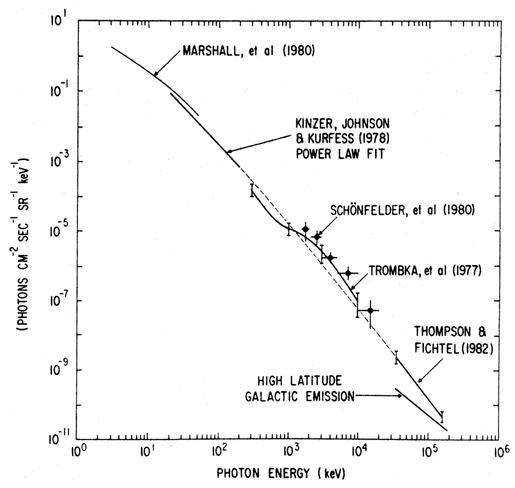
\includegraphics[width = 0.70\textwidth]{gamma_ray_background_spectrum.png}
\caption{Gamma-ray background surface brightness spectrum (From Trombka and Fichtel 1983).}
\end{center}
\end{figure}

\end{document}
